\documentclass{beamer}
\usetheme{Madrid}
\usecolortheme{default}

\title[Baseball Analytics Using Machine Learning]
{Baseball Analytics Using Machine Learning}

\subtitle{ECE1513}

\author[Mia Cong, Spiro Li, Jacky Lai] 
{Yuan (Mia) Cong\inst{1} \and Spiro Li\inst{2} \and Jacky Lai\inst{3}}

\institute[ ] % (optional)
{
  \inst{1}%
  Department of Mechanical \& Industrial Engineering
  \and
  \inst{2}%
  Department of Electrical and Computer Engineering
  \and
   \inst{3}%
  Department of Mechanical \& Industrial Engineering
}

\date[IntroML] % (optional)
{Introduction to Machine Learning -- Winter 2026}

\logo{\includegraphics[height=0.8cm]{logo_uoft}}

\definecolor{uoftblue}{RGB}{6,41,88}
\setbeamercolor{titlelike}{bg=uoftblue}
\setbeamerfont{title}{series=\bfseries}

\usepackage{graphicx}
\usepackage{tikz}
\usepackage{xcolor}
\begin{document}

\frame{\titlepage}
\setcounter{framenumber}{0}

\begin{frame}[t]
\frametitle{Problem \& Dataset}

\vspace{-2pt}
{\small\textbf{Goal:} Predict team wins in season $t$ from previous-season stats --- \textbf{supervised regression}.}

\vspace{5pt}
\begin{columns}[T]

% ════ LEFT COLUMN ════
\begin{column}{0.47\textwidth}

\begin{block}{\scriptsize Dataset}
\vspace{-4pt}
{\scriptsize
\begin{itemize}
  \setlength{\itemsep}{0pt}
  \item \textbf{Lahman Baseball Database} --- \texttt{Teams}
  \item ${\sim}$30 teams/yr $\times$ ${\sim}$20 seasons $\approx$ \textbf{600 rows}
  \item Years 2000--2025, \textbf{excl.\ 2020} (COVID)
\end{itemize}
}
\vspace{-4pt}
\end{block}

\vspace{2pt}
{\scriptsize\textbf{Temporal split} (no data leakage)}\\[1pt]
{\scriptsize
\begin{tabular}{@{}ll@{}}
  \textbf{Train:} & 2001--2019 (${\sim}$570 rows) \\
  \textbf{Test:}  & 2021--2025 (${\sim}$150 rows) \\
\end{tabular}}\\[1pt]
{\tiny\color{gray}\itshape Features lagged one season per franchise.}

\vspace{5pt}
{\scriptsize\textbf{Pipeline} (increasing complexity)}
\vspace{-1pt}
{\scriptsize
\begin{enumerate}
  \setlength{\itemsep}{2pt}
  \item Pythagorean expectation $\left(\text{Win\%} = \frac{R^2}{R^2 + \text{RA}^2}\right)$ {\color{gray}\itshape-- no learning}
  \item Ridge Regression {\color{gray}\itshape-- linear}
  \item SVR {\color{gray}\itshape-- kernel}
  \item Neural Network {\color{gray}\itshape-- deep}
\end{enumerate}
}

\end{column}

% ════ RIGHT COLUMN ════
\begin{column}{0.50\textwidth}

\begin{block}{\scriptsize 15 Features (previous-season stats)}
\vspace{-2pt}
{\scriptsize

\textbf{Batting (7)}\\[1pt]
\begin{tabular}{@{}l@{\;}l@{\qquad}l@{\;}l@{}}
  R  & Runs scored  & BB  & Walks \\
  H  & Hits         & SO  & Strikeouts \\
  HR & Home runs    & SB  & Stolen bases \\
     &              & HBP & Hit by pitch \\
\end{tabular}

\vspace{3pt}
\textbf{Pitching (6)}\\[1pt]
\begin{tabular}{@{}l@{\;}l@{\qquad}l@{\;}l@{}}
  RA  & Runs allowed   & BBA & Walks allowed \\
  ERA & Earned run avg & SOA & Strikeouts (P) \\
  HA  & Hits allowed   & HRA & HR allowed \\
\end{tabular}

\vspace{3pt}
\textbf{Fielding (2)}\\[1pt]
\begin{tabular}{@{}l@{\;}l@{\qquad}l@{\;}l@{}}
  E  & Errors & FP & Fielding pct \\
\end{tabular}

}
\vspace{-2pt}
\end{block}

\end{column}
\end{columns}

\end{frame}


\begin{frame}
\frametitle{Slide 2}

In this slide, some important text will be
\alert{highlighted} because it's important.
Please, don't abuse it.

\begin{block}{Remark}
Sample text
\end{block}

\begin{alertblock}{Important theorem}
Sample text in red box
\end{alertblock}

\begin{examples}
Sample text in green box. The title of the block is ``Examples".
\end{examples}
\end{frame}

\begin{frame}[t]
\frametitle{Neural Network Results}
 
\vspace{-2pt}
{\scriptsize\color{gray}%
FNN ~$\cdot$~ 15\,$\to$\,64\,$\to$\,32\,$\to$\,1 ~$\cdot$~ 3,137 params ~$\cdot$~ ReLU + linear output ~$\cdot$~ MSE loss ~$\cdot$~ Adam}
 
\vspace{2pt}
\begin{columns}[T]
 
% ── LEFT COLUMN ──
\begin{column}{0.47\textwidth}
{\small\textbf{Training curve}}
 
\vspace{2pt}
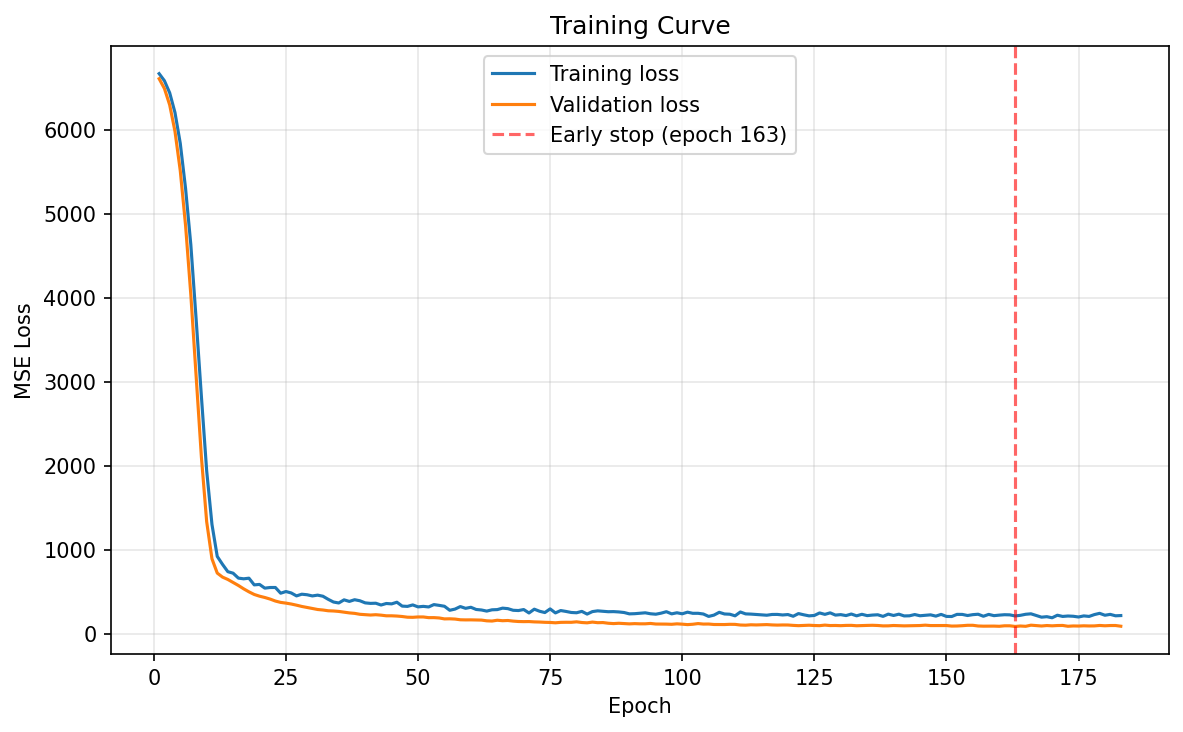
\includegraphics[width=\textwidth]{../results/neural_net/training_curve.png}
 
\vspace{1pt}
{\tiny\itshape\color{gray}%
Early stopped at epoch 249 / 269 --- no overfitting gap}
 
\vspace{4pt}
{\scriptsize
\begin{itemize}
  \setlength{\itemsep}{1pt}
  \item Mini-batch SGD ($B\!=\!32$) + Adam
  \item Weight decay $\lambda\!=\!10^{-4}$, Dropout $p\!=\!0.2$
  \item ${\sim}$570 train samples, 15\% for validation
\end{itemize}
}
\end{column}
 
% ── RIGHT COLUMN ──
\begin{column}{0.50\textwidth}
 
\begin{block}{\scriptsize vs.\ Pythagorean baseline (no learning)}
\centering\vspace{2pt}
\begin{columns}[c]
\begin{column}{0.45\linewidth}
\centering
{\tiny\color{gray}MAE}\\[1pt]
{\Large\textbf{\color{teal}9.85}}\\[1pt]
{\tiny\color{gray}vs 10.73}
\end{column}
\begin{column}{0.45\linewidth}
\centering
{\tiny\color{gray}RMSE}\\[1pt]
{\Large\textbf{\color{teal}12.59}}\\[1pt]
{\tiny\color{gray}vs 13.48}
\end{column}
\end{columns}
\vspace{2pt}
\end{block}
 
\vspace{2pt}
{\small\textbf{Predicted vs.\ actual (test set)}}
 
\vspace{2pt}
\begin{columns}[c]
\begin{column}{0.60\linewidth}
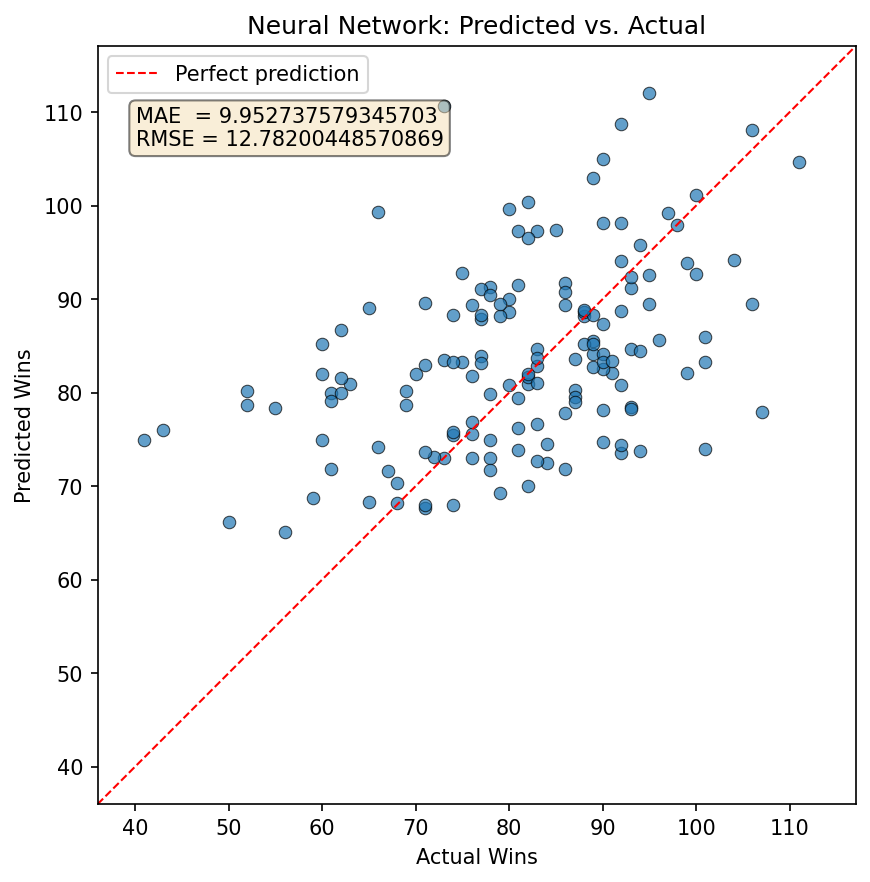
\includegraphics[width=\textwidth]{../results/neural_net/nn_pred_vs_actual.png}
\end{column}
\begin{column}{0.36\linewidth}
\centering
\colorbox{teal!10}{%
\parbox{2cm}{\centering\vspace{3pt}
{\small\textbf{\color{teal}${\sim}$8\% MAE}}\\
{\small\textbf{\color{teal}improvement}}\\[2pt]
{\tiny\color{gray}over no-learning}\\
{\tiny\color{gray}baseline}
\vspace{3pt}}}
\end{column}
\end{columns}
 
\end{column}
\end{columns}
 
\end{frame}

\begin{frame}[t]
\frametitle{SVR Results}

\vspace{-2pt}
{\scriptsize\color{gray}%
SVR ~$\cdot$~ kernels: linear / RBF ~$\cdot$~ GridSearchCV (MAE) ~$\cdot$~ best: linear, $C=0.1$, $\epsilon=0.1$}

\vspace{0pt}
\setlength{\columnsep}{2pt}
\begin{columns}[T,totalwidth=\textwidth]

% ── LEFT COLUMN ──
\begin{column}{0.495\textwidth}
{\scriptsize\textbf{Kernel comparison (CV MAE)}}

\vspace{0pt}
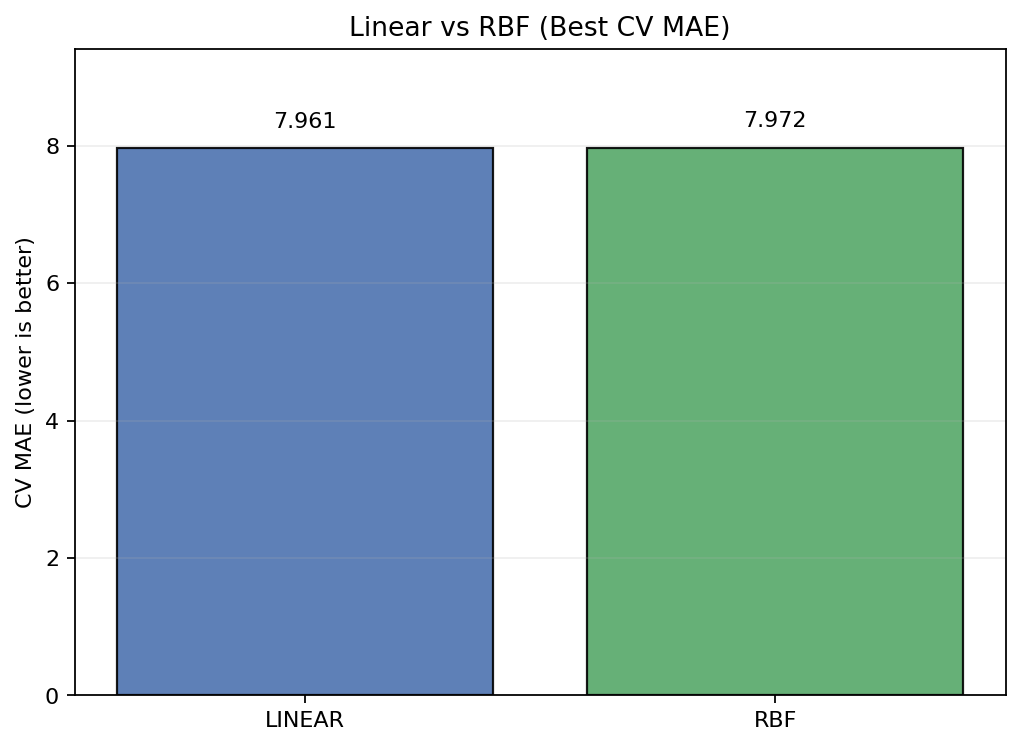
\includegraphics[width=\textwidth,height=0.30\textheight,keepaspectratio]{../results/svr/svr_kernel_cv_mae.png}

\vspace{0pt}
{\scriptsize\textbf{Residual distribution (test set)}}

\vspace{-1pt}
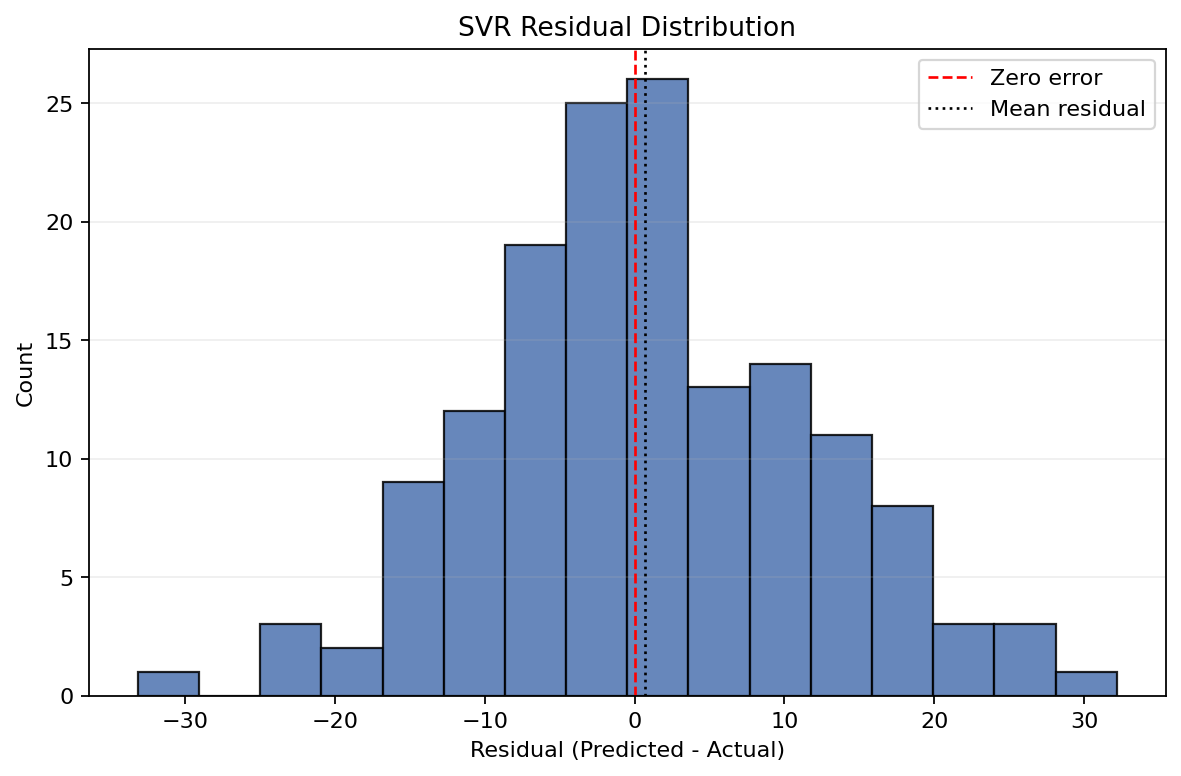
\includegraphics[width=\textwidth,height=0.28\textheight,keepaspectratio]{../results/svr/svr_residual_hist.png}
\end{column}

% ── RIGHT COLUMN ──
\begin{column}{0.495\textwidth}

\begin{block}{\tiny vs.\ Pythagorean baseline (no learning)}
\centering\vspace{-1pt}
\begin{columns}[c]
\begin{column}{0.45\linewidth}
\centering
{\tiny\color{gray}MAE}\\[0pt]
{\small\textbf{\color{teal}8.52}}\\[-1pt]
{\scriptsize\color{gray}vs 10.73}
\end{column}
\begin{column}{0.45\linewidth}
\centering
{\tiny\color{gray}RMSE}\\[0pt]
{\small\textbf{\color{teal}10.98}}\\[-1pt]
{\scriptsize\color{gray}vs 13.48}
\end{column}
\end{columns}
\vspace{-1pt}
\end{block}

\vspace{-4pt}
{\scriptsize\textbf{Predicted vs.\ actual (test set)}}

\vspace{-1pt}
\begin{columns}[c]
\begin{column}{0.69\linewidth}
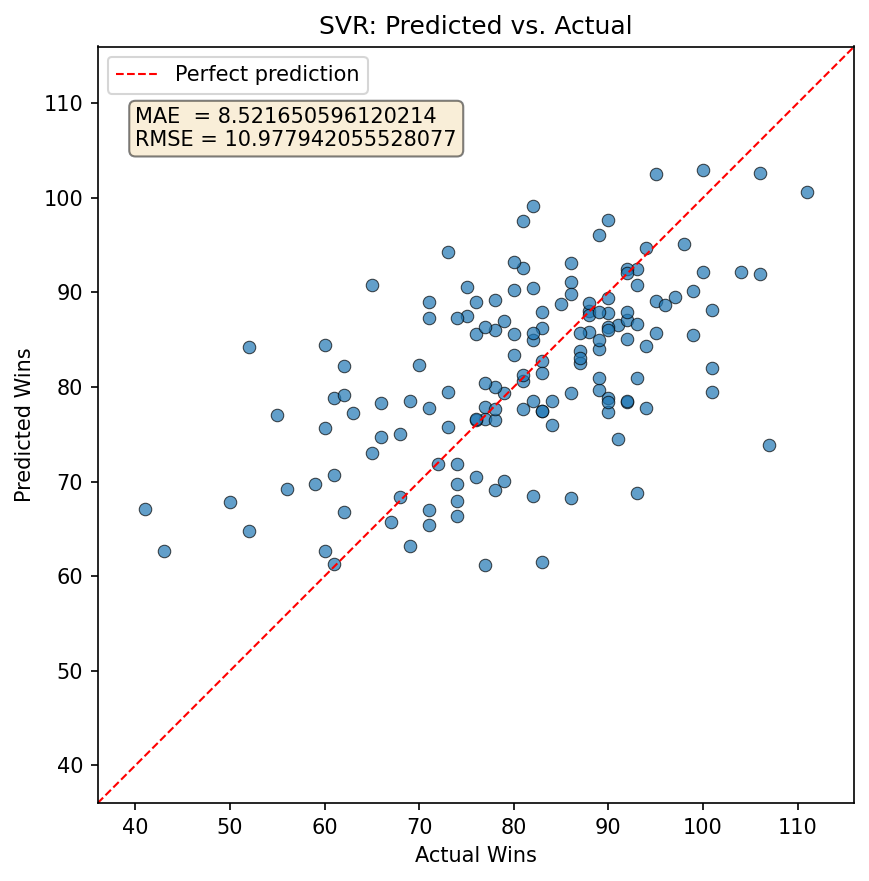
\includegraphics[width=\textwidth,height=0.44\textheight,keepaspectratio]{../results/svr/svr_pred_vs_actual.png}
\end{column}
\begin{column}{0.29\linewidth}
\centering
\colorbox{teal!10}{%
\parbox{1.95cm}{\centering\vspace{2pt}
{\scriptsize\textbf{\color{teal}${\sim}$21\% MAE}}\\
{\scriptsize\textbf{\color{teal}improve}}\\[-1pt]
{\scriptsize\textbf{\color{teal}ment}}\\[2pt]
{\tiny\color{gray}over no-learning}\\
{\tiny\color{gray}baseline}
\vspace{2pt}}}
\end{column}
\end{columns}

\end{column}
\end{columns}

\end{frame}

\end{document}